%Stanford, August 14, 2016
\documentclass[10pt,compress,xcolor={usenames,dvipsnames}]{beamer} %slides and notes
\usepackage{amsmath,datetime,xmpmulti,mathtools,bbm,array,booktabs,alltt,xspace,mathabx,pifont,tikz,calc,colortbl,stmaryrd,graphicx}
\usepackage[usenames]{xcolor}
\usepackage[tikz]{mdframed}
\usepackage[author-year]{amsrefs}
\usepackage{newpxtext}
%\usepackage{newtxtext}
%\usepackage{newtxmath}
\usepackage[euler-digits,euler-hat-accent]{eulervm}
\usetikzlibrary{arrows}
\usepackage{cleveref}
\usetheme{FJHSlimNoFoot}

\definecolor{ltred}{rgb}{1,0.75,0.75}

\setlength{\parskip}{2ex}
\setlength{\arraycolsep}{0.5ex}

\makeatletter
\newcommand{\vast}{\bBigg@{3}}
%\newcommand{\vast}{\bBigg@{4}}
\newcommand{\Vast}{\bBigg@{5}}
\makeatother


\mdfdefinestyle{redshade}{%
	leftmargin=0 pt,
	rightmargin = 0pt,
	innerleftmargin = 1ex,
	innerrightmargin = 1ex,
	skipabove = 0 pt,
	skipbelow = 0 pt,
	backgroundcolor=red!20,
	linecolor=red!20,
	roundcorner=5pt}

\title[]{Error Analysis for Quasi-Monte Carlo Methods}
\author[]{Fred J. Hickernell}
\institute{Department of Applied Mathematics,  Illinois Institute of Technology \\
\href{mailto:hickernell@iit.edu}{\url{hickernell@iit.edu}} \quad
\href{http://mypages.iit.edu/~hickernell}{\url{mypages.iit.edu/~hickernell}}}
\thanksnote{Thanks to the Guaranteed Automatic Integration Library (GAIL) team  and friends\\[1.5ex]
	Supported by NSF-DMS-1522687\\[1.5ex]
	Thanks to the MCQMC 2016 organizers}
\date[]{MCQMC \textbullet\ August 14, 2016}

%Title:  Guaranteed Fixed-Width Confidence Intervals for Monte Carlo and Quasi-Monte Carlo Simulation

%Abstract: When performing a simulation to determine $\mu=\mathbb{E}(Y)$ one wonders what the error is and how many samples are required to achieve a desired accuracy.  We may want a confidence interval for the of the form $\mathbb{P}[\lvert\mu - \hat{\mu}_n\rvert\le \varepsilon] \ge 99\%$ where $\varepsilon$ is fixed by the user, and the number of samples, $n$, must be determined to make the sample mean, $\hat{\mu}_n$ close enough to the true mean.  Popular confidence intervals are based on large sample results, such as the Central Limit Theorem, or heuristics, but these error estimates can be fooled.  We explain how these popular estimates can fail and present new, guaranteed, fixed-width confidence intervals for  simple Monte Carlo and quasi-Monte Carlo simulation.   Moreover, we provide upper bounds on the required sample sizes  that show a reasonable dependence on the unknown difficulty of the simulation.



\input FJHDef.tex
\renewcommand{\mSigma}{\Sigma}
\newcommand{\smallcite}[1]{{\small\cite{#1}}}
\newcommand{\smallocite}[1]{{\small\ocite{#1}}}
\newcommand{\smallcites}[1]{{\small\cites{#1}}}
\newcommand{\tol}{\text{tol}}
\newcommand{\Phnu}{\Prob_{\hnu}}
\DeclareMathOperator{\hugetext}{huge}
\DeclareMathOperator{\oerr}{\overline{err}}
\DeclareMathOperator{\cubMC}{cubMC}
\DeclareMathOperator{\qse}{qse}
\DeclareMathOperator{\integ}{int}
\DeclareMathOperator{\trap}{trap}
\DeclareMathOperator{\size}{size}
\DeclareMathOperator{\app}{id}
\DeclareMathOperator{\err}{err}
\DeclareMathOperator{\MSE}{MSE}
\DeclareMathOperator{\RMSE}{RMSE}
\DeclareMathOperator{\PProb}{\mathbb{P}}
\DeclareMathOperator{\walsh}{walsh}
\newcommand{\happ}{\widehat{\app}}
\newcommand{\hinteg}{\widehat{\integ}}
\newcommand{\cube}{[0,1)^d}
\newcommand{\desall}{\{\vz_i\}}
\newcommand{\desn}{\{\vz_i\}_{i=0}^{n-1}}
\def\newblock{\hskip .11em plus .33em minus .07em}
\newcommand{\wcS}{\widecheck{S}}
\newcommand{\wcomega}{\widecheck{\omega}}
\newcommand{\HickernellFJ}{H.} %To give my name to the bibliography
\newcommand{\abstol}{\varepsilon_{\text{a}}}
\newcommand{\reltol}{\varepsilon_{\text{r}}}
\DeclareMathOperator{\MLE}{MLE}
\DeclareMathOperator{\algn}{ALN}
\DeclareMathOperator{\disc}{DSC}
\DeclareMathOperator{\Var}{VAR}
\DeclareMathOperator{\RMS}{RMS}
\DeclareMathOperator{\GP}{\cg\cp}
\newcommand{\Dt}{\text{D}}
\newcommand{\Rn}{\text{R}}
\newcommand{\Ba}{\text{B}}
\newcommand{\tmC}{\widetilde{\mC}}
\newcommand{\tvC}{\widetilde{\vC}}
\newcommand{\vC}{\boldsymbol{C}}
\newcommand{\hvtheta}{\hat{\vtheta}}
\newcommand{\hs}{\hat{s}}

\newcommand{\redroundmathbox}[1]{\parbox{\widthof{$#1$\hspace{1em}}}
	{\begin{mdframed}[style=redshade]\centering $#1$ \end{mdframed}}}
\newcommand{\setbeameruncoveredtransp}{\setbeamercovered{transparent=10}}
\newcommand{\shadegraph}[1]{\tikz\node[opacity=0.25, inner sep=0, outer sep=0]{#1};}
\newcommand{\sleepPict}{\href{http://www.preapps.com/blog/wp-content/uploads/2015/09/Valuable-Sleep.jpg}{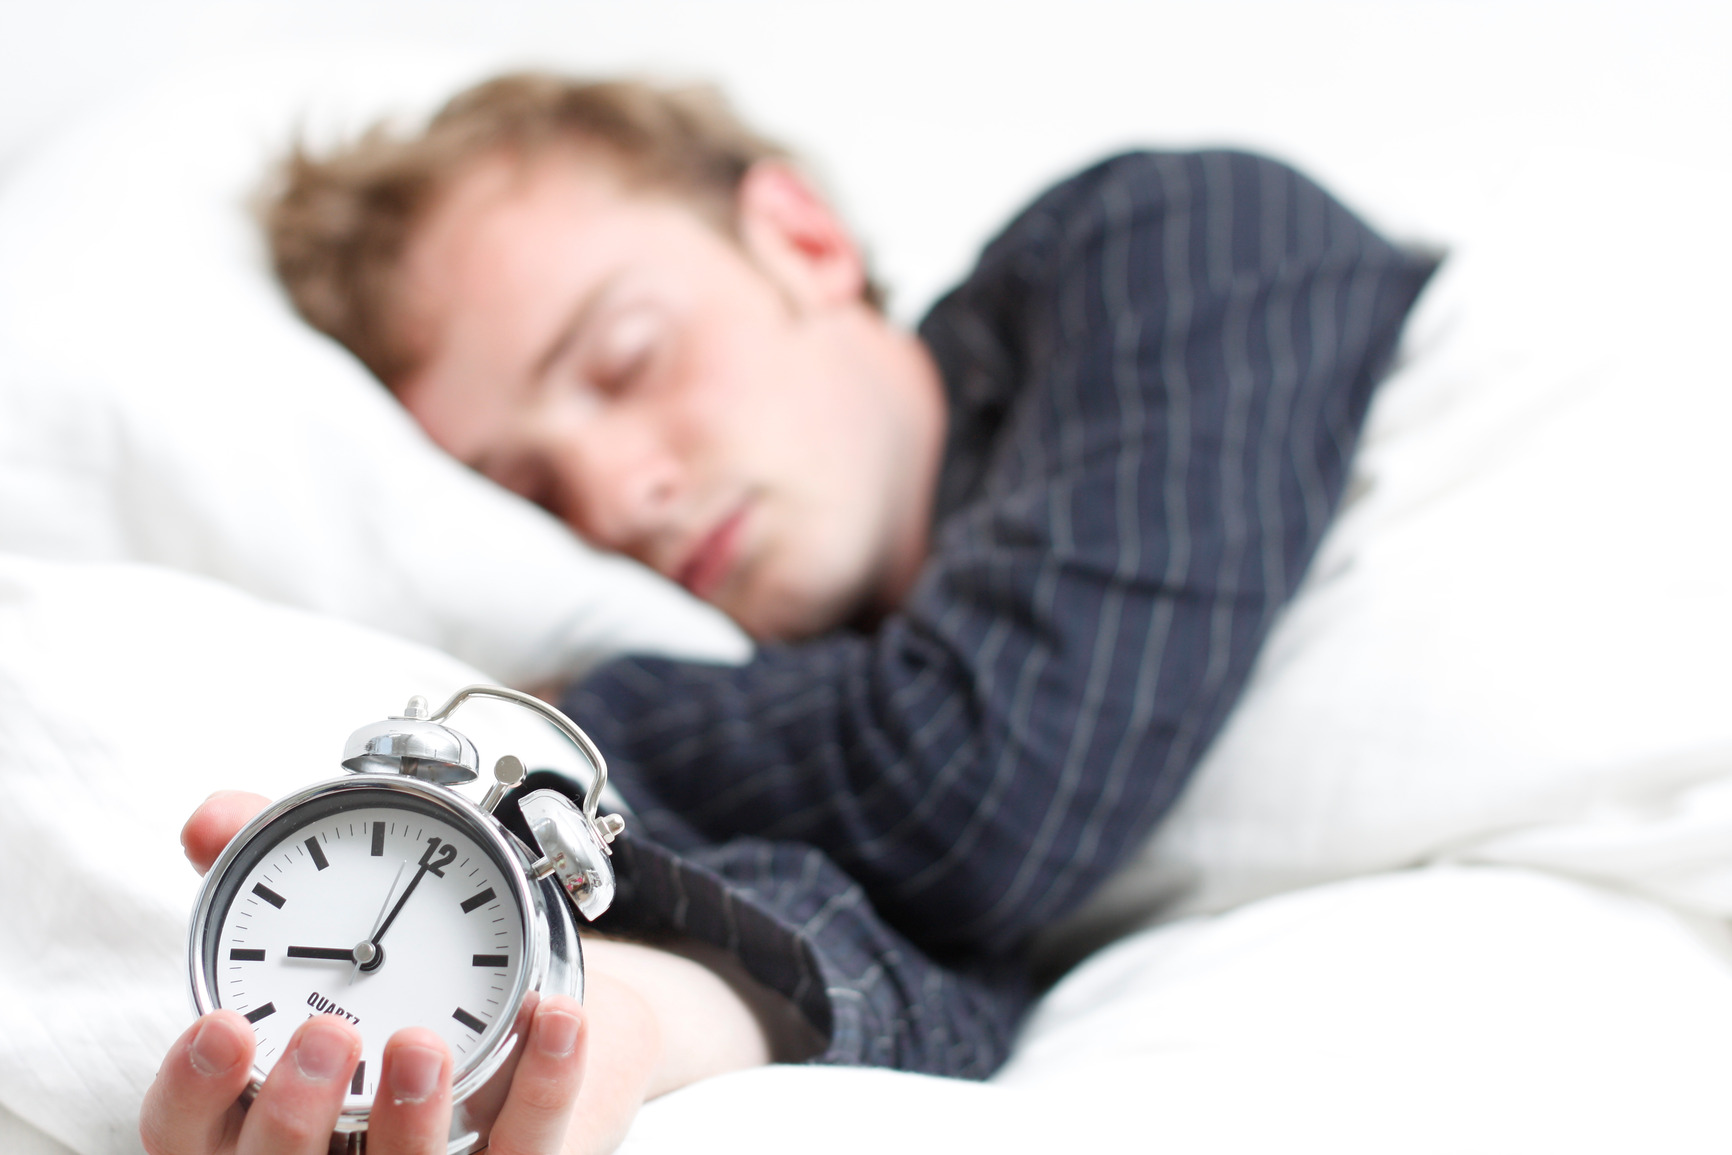
\includegraphics[width = 3cm]{ProgramsImages/Valuable-Sleep.jpg}}}
\newcommand{\financePict}{\href{http://i2.cdn.turner.com/money/dam/assets/130611131918-chicago-board-options-exchange-1024x576.jpg}{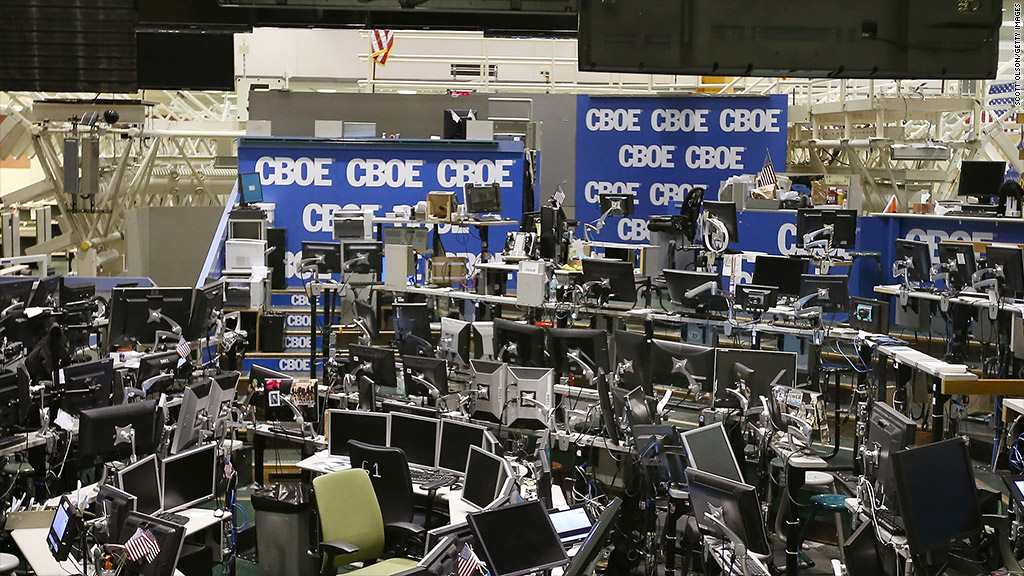
\includegraphics[width = 3cm]{ProgramsImages/130611131918-chicago-board-options-exchange-1024x576.jpg}}}
\newcommand{\GaussPict}{\href{http://www.mathworks.com/matlabcentral/answers/uploaded_files/26298/Plotting\%20a\%203d\%20gaussian\%20function\%20using\%20surf\%20-\%202015\%2002\%2027.png}{\includegraphics[width = 3cm]{ProgramsImages/Plotting_gaussian.png}}}

\newcommand{\medcone}{\parbox{1.2cm}{\includegraphics[width=0.55cm,angle=270]{ProgramsImages/MediumWaffleCone.eps}}\xspace}

\newcommand{\smallcone}{\parbox{0.65cm}{\includegraphics[width=0.3cm,angle=270]{ProgramsImages/MediumWaffleCone.eps}}\xspace}

\newcommand{\lecone}{\smallcone\hspace*{-0.3cm}\mathclap{\le}\hspace*{0.35cm}}

\definecolor{MATLABBlue}{rgb}{0, 0.447, 0.741}
\definecolor{MATLABOrange}{rgb}{0.85,  0.325, 0.098}
\definecolor{MATLABPurple}{rgb}{0.494,  0.184, 0.556}
\definecolor{MATLABGreen}{rgb}{0.466,  0.674, 0.188}



\begin{document}
\tikzstyle{every picture}+=[remember picture]
\everymath{\displaystyle}

\frame{\titlepage}

\section{Motivation}

\begin{frame}
	%\setbeameruncoveredtransp
	\frametitle{\textbf<1>{Error Analysis} for \textbf<2>{Quasi-Monte Carlo Methods}}
	\vspace{-7ex}
{\large	\begin{gather*} \mu := \Ex[f(\vX)] := \int_{\cx} f(\vx) \, \nu(\dif\vx) \approx \hmu := \sum_{i=1}^n f(\vx_i) w_i = \int_{\cx} f(\vx) \, \hnu(\dif\vx) \\
	\redroundmathbox{\mu - \hmu = \int_{\cx} f(\vx) \, (\nu - \hnu)(\dif\vx) =\, ?} 
	 \end{gather*}
	 \vspace{-7ex}
	\begin{center}
		\begin{tabular}{>{\centering}p{0.45\textwidth}>{\centering}p{0.5\textwidth}}
\uncover<1->{\alert{Reality} & \alert{\textbf<1>{Error Analysis} (Theory)} \tabularnewline 
What is &  What we think it should be \\ by rigorous argument \\[1ex]}
Not certain that \\
our assumptions hold
		\end{tabular}
	\end{center}
\uncover<2->{\alert{\textbf<2>{Quasi-Monte Carlo Methods}} \\ [-1ex]
	\begin{itemize}
		\item $w_1  = \cdots = w_n = 1/n$ or
		\item $\vx_i$ chosen carefully
	\end{itemize}}}
\end{frame}
 
\begin{frame}
	\setbeameruncoveredtransp
	\frametitle{Integration Examples}
	\vspace{-8ex}
	\begin{tabular}{m{8cm}m{3cm}}
	\[ \begin{aligned}
	\mu &= \frac{1}{N} \sum_{j=1}^N f(j) = \text{population average hours of sleep} \\ f(j) & = \text{hours of sleep for individual } j 
	\end{aligned} \]
	& \sleepPict
\uncover<2->{
	\tabularnewline [-2.2ex] \arrayrulecolor{ltred}\toprule
\tabularnewline [-1.5ex] 
\vspace{-4ex}
		\[ \begin{aligned} \mu &= \int_{\reals^d} f(\vx) \, \nu (\dif \vx) =  \text{option price}\\ f(\vx) & = \text{discounted payoff determined by innovations }\vx
			\end{aligned} \] 
		& \vspace{-2ex}
		\only<1>{\shadegraph{\financePict}}\only<2->{\financePict}}
	 \uncover<3->{
	 	\tabularnewline[-1ex] \arrayrulecolor{ltred}\toprule
\tabularnewline [-3ex] 
\vspace{-2ex}
	 	\[ \begin{aligned}\mu &= \int_{\cx} g(\vx) \, \dif \vx = \Prob(\vX \in \cx) = \text{probability} \\ g & = \text{probability density function}
	 		\end{aligned} \] 
	 		& \vspace{-1ex} \only<1-2>{\shadegraph{\GaussPict}}\only<3->{\GaussPict}} 
	 	\tabularnewline[-2ex]  \arrayrulecolor{ltred}\toprule
\end{tabular}
	\vspace{-1ex}
\begin{gather*}
	 	\mu  = \Ex[f(\vX)] = \int_{\cx} f(\vx) \, \nu(\dif\vx) \approx \hmu = \sum_{i=1}^n f(\vx_i) w_i = \int_{\cx} f(\vx) \, \hnu(\dif\vx)
	 				\qquad \redroundmathbox{\mu - \hmu =\, ?} \\
	 	\nu = \text{probability measure}, \quad\hnu = \sum_{i=1}^n w_i \delta_{\vx_i} = \text{sampling measure},\quad \sum_{i=1}^n w_i =1
	 	\end{gather*}
\end{frame}


\section{Trio Error Identity}

\begin{frame}
	\setbeameruncoveredtransp
	\frametitle{Trio Identity for the Error {\large \cite{Men16a}}}
	\vspace{-7ex}
	\begin{align*}
	 \redroundmathbox{\mu - \hmu} &= \int_{\cx} f(\vx) \, \nu(\dif\vx) - \sum_{i=1}^n f(\vx_i) w_i = \int_{\cx} f(\vx) \, (\nu - \hnu)(\dif\vx) \\
	&=  \redroundmathbox{\algn(f,\nu - \hnu) \, \disc(\nu - \hnu) \, \Var(f)} \\[1ex]
   \Var(f) & =  \text{\alert{variation} of the integrand} \ge 0 \\
	\disc(\nu - \hnu) & =  \text{\alert{discrepancy} of the sampling measure }\\
	 &  \qquad \qquad  \text{from the probability measure} \ge 0\\
	\algn(f,\nu - \hnu) & =  \text{\alert{alignment} of the integrand and} \\
	&  \qquad \qquad  \text{the difference between the two measures}
\only<1>{\\ & \hspace{3cm} \qquad \text{\alert{often ignored, but shouldn't be}}}
	\end{align*}
			
	\uncover<2>{\vspace{1ex}\centerline{\begin{tabular}{r@{\quad}@{\quad}c@{\qquad}c}
		\multicolumn{1}{c}{}& \multicolumn{2}{c}{Sampling Distribution, $\hnu$}\\
		 Integrand, $f$ & Fixed & Random \\  \cmidrule[1.5pt]{2-3} \\   [-1ex]
		 Fixed & Deterministic & Randomized \\ [1ex]
		Gaussian Process	& Bayesian & Bayesian Randomized	
	\end{tabular}}}

\end{frame}

\begin{frame}
	\setbeameruncoveredtransp
	\frametitle{Deterministic Trio Identity}
	\vspace{-8ex}
	\begin{align*}
	(\cf, \norm[\cf]{\cdot}) & = \text{normed vector space of integrands} \\
	& \qquad f \mapsto f(\vx) \text{ is bounded for all } \vx \in \cx \\
	(\cm, \norm[\cm]{\cdot}) & = \text{normed vector space of signed measures} \\
	& \qquad  \norm[\cm]{\lambda} := \sup_{0 \ne f \in \cf} \frac{\abs{\int_{\cx} f(\vx) \, \lambda(\dif\vx)}}{\norm[\cf]{f}} \\
\redroundmathbox{\mu - \hmu} &= \int_{\cx} f(\vx) \, (\nu - \hnu)(\dif\vx) \\
	\uncover<2->{	& =  \redroundmathbox{%
		\underbrace{\frac{ \int_{\cx} f(\vx) \, (\nu - \hnu)(\dif\vx)}{\norm[\cm]{\nu - \hnu} \norm[\cf]{f-L(f)}}}_{\textstyle \algn^\Dt(f,\nu - \hnu)} \, \underbrace{\norm[\cm]{\nu - \hnu}}_{\textstyle\disc^\Dt(\nu - \hnu)} \, \underbrace{\norm[\cf]{f}}_{\textstyle\Var^\Dt(f)}}}
	\end{align*}
	\vspace{-4ex}
	\uncover<2->{\begin{itemize}
			\item $\abs{\algn^\Dt(f,\nu - \hnu)}   \le 1$  %by the definitions of $\norm[\cf]{\cdot}, \norm[\cm]{\cdot}$
			\item Ignoring $\algn^\Dt(f,\nu - \hnu)$ yields a generalized Koksma-Hlawka inequality \cites{Hla61, Nie92,Hic97a,Hic99a}
		\end{itemize}.}
\end{frame}

\begin{frame}
	\frametitle{Hours of Sleep Web Survey}
	\vspace{-8ex}
	\begin{tabular}{m{8cm}m{3.5cm}}
		\begin{gather*}
		\mu %= \frac 1N \sum_{j=1}^N f(j) 
		= \text{population average hours of sleep}  \\
		f(j) = \text{hours of sleep for individual } j \\
			\nu = \text{uniform}, \qquad \hnu  = \frac 1n \sum_{i=1}^n \delta_{x_i}\\
			\{x_i\}_{i=1}^n \text{is a sequence of distinct individuals}
			\end{gather*}
			& \sleepPict
	\end{tabular}
	\vspace{-4ex}
\[ \mu = \mu(f) = \frac 1N \sum_{j=1}^N f(j) , \qquad \cov(f,g) = \frac 1N \sum_{i=1}^N [f(j) - \mu(f)][g(j) - \mu(g)]\]
	\centerline{\redroundmathbox{\mu - \hmu  = 
			\underbrace{-\corr\bigl(f, \bbone_{\{\vx_i\}_{i=1}^n}\bigr)}_{\textstyle\algn^\Dt(f,\nu - \hnu)}
			\underbrace{ \sqrt{\frac{1-n/N}{\alert{n/N}}}}_{\textstyle\disc^\Dt(\nu - \hnu)}
			\underbrace{ \std(f)}_{\textstyle\Var^\Dt(f)} }}
		\vspace{-2ex}
		\begin{itemize}
			\item Discrepancy depends on the \alert{sample fraction}, not merely the sample size  \smallcite{Men16a}
						
			\item \alert{Correlation} for a web survey is difficult to predict or control
		\end{itemize}
\end{frame}

\begin{frame}
	\frametitle{Reproducing Kernel Hilbert Spaces (RKHS)}
	\vspace{-4ex}
	If the space of integrands, $\cf$ is a Hilbert space with \alert{reproducing kernel} $K:\cx \times \cx \to \reals$, then the \alert{cubature error} is the \alert{inner product} of the integrand with the representer for the error functional \smallcite{Hic99a}:
	\begin{align*}
	\Var(f) &= \norm[\cf]{f}, \qquad f(\vt) = \ip[\cf]{K(\cdot,\vt)}{f} \ \forall \vt \in \cx,\ f \in \cf\\
	[\disc(\nu - \hnu)]^2 &  =  \int_{\cx^2}K(\vx, \vt) \, \nu(\dif \vx) \nu(\dif \vt) - 2 \sum_{i=1}^n w_i \int_{\cx} K(\vx_i, \vt) \, \nu(\dif \vt) \\
	& \qquad \qquad + \sum_{i,j=1}^n w_i w_j K(\vx_i, \vx_j) \\
	\algn(f,\nu - \hnu)  &= \cos\biggl(f,\underbrace{\int_{\cx} K(\cdot, \vt) \, \nu(\dif \vt) + \sum_{j=1}^n w_j K(\cdot, \vx_j)}_{\textstyle\text{cubature error representer}}\biggr), \\ & \qquad \qquad \cos(f,g) : = \frac{\ip[\cf]{f}{g}}{\norm[\cf]{f} \norm[\cf]{g}}
	\end{align*}
	\centerline{\redroundmathbox{\mu - \hmu = \cos(f,\text{error rep}) \disc^\Dt(\nu - \hnu) \norm[\cf]{f}}
	}
\end{frame}

\begin{frame}
	\frametitle{$L^2$-Discrepancy}
	\vspace{-9ex}
	\begin{align*}
	\cx &= [0,1]^d, \qquad  \nu = \text{uniform}, \qquad K(\vx,\vt) =\prod_{k = 1}^d [2 - \max(x_k,t_k)] \\[-1ex]
	\Var^\Dt(f) & = \norm[\cf]{f-f(\vone)} = \Bigl \lVert \bigl ( \norm[L^2]{\partial^\fu f}\bigr )_{\emptyset \ne \fu \subseteq 1:d} \Bigr \rVert_2 , \qquad 
	\partial^\fu f : = \frac{\partial^{\abs{\fu}} f}{\partial \vx_\fu} \biggr \rvert_{\textstyle \vx_{\widebar{\fu}} = \vone} \\
	[\disc^\Dt(\nu - \hnu)]^2 &  = \left(\frac 43\right)^d - 2 \sum_{i=1}^n w_i \prod_{k=1}^d \left (\frac{3 - x_{ik}^2}{2} \right) + \sum_{i,j=1}^n w_i w_j \prod_{k = 1}^d [2 - \max(x_{ik},x_{jk})] 
	\only<2->{\\& = \Bigl \lVert \bigl ( \norm[L^2]{\nu([\vzero,\cdot_\fu]) - \hnu([\vzero,\cdot_\fu])}\bigr )_{\emptyset \ne \fu \subseteq 1:d} \Bigr \rVert_2}
	\end{align*}
	\only<1>{\vspace*{-1.8ex}
		\centerline{\includegraphics[width = 7cm]{ProgramsImages/L2Kernel.eps}}}
	\only<2>{\begin{tabular}{>{\flushright}m{5cm}>{\centering}m{6cm}}
			$ \vx = (\ldots, 0.6, \ldots, 0.4, \ldots)$
			\begin{multline*}
			\nu([\vzero,\vx_{\{5,8\}}]) - \hnu([\vzero,\vx_{\{5,8\}}]) \\
			 = 0.24 - 7/32 = 0.02125
			\end{multline*}& \vspace{-1ex}
			\includegraphics[width = 4.4cm]{ProgramsImages/LocalDiscrep.eps}
		\end{tabular}}
\only<3>{	\centerline{\redroundmathbox{\mu - \hmu = \cos(f,\text{error rep}) \disc^\Dt(\nu - \hnu) \norm[\cf]{f-f(\vone)}}}
	\vspace{-4ex}
	\begin{itemize}
		\item $\disc^\Dt(\nu - \hnu)$ requires $\Order(dn^2)$ operations to evaluate
		\item $\disc^\Dt(\nu - \hnu) \begin{cases} =  \Order(n^{-1/2}) \text{ for IID Monte Carlo} \\
		= \Order( n^{\alert{-1} + \epsilon}) \text{ for digital nets, integration lattices, \ldots} \\
		\qquad \qquad \text{\smallcites{Nie92, DicPil10a}} \\
		\ge \Order(n^{\alert{-1} + \epsilon}) \text{ because of the limited smoothness of } f \in \cf\end{cases}$
	\end{itemize}
	\vspace{-2ex}
	\qquad \alert{Low discrepancy (quasi-Monte Carlo) sampling reduces cubature error}}
\end{frame}


\begin{frame} \frametitle{Multivariate Normal Probability}
	\vspace{-8ex}
	\begin{tabular}{m{8.5cm}m{3cm}}
	\begin{gather*}
	\mu = \int_{[\va,\vb]} \frac{\exp\bigl(- \frac 12 \vt^T \mSigma^{-1} \vt \bigr)}{\sqrt{(2 \pi)^d \det(\mSigma)}} \, \dif \vt \
	\overset{\text{\smallocite{Gen93}}}{=} \ \int_{[0,1]^{d-1}} f(\vx) \, \dif \vx \\
		\hnu = \text{equally weighted average}
		\end{gather*}
		& \GaussPict
	\end{tabular}
	\vspace{-4ex}
	
		\centerline{\redroundmathbox{\mu - \hmu = \cos(f,\text{error rep}) \disc^\Dt(\nu - \hnu) \norm[\cf]{f-f(\vone)}}}
		
		\vspace{-2ex}
\begin{tabular}{m{4.5cm}m{7cm}}
	\vspace{-4ex}
\[\begin{aligned}\MoveEqLeft \disc^\Dt(\nu - \hnu) \\
& \begin{cases} =  \Order(n^{-1/2}) \text{ for IID MC}\\
		= \Order( n^{\alert{-1} + \epsilon}) \text{ for Sobol'}
		\end{cases}
	\end{aligned} \] 
	\vspace{2ex}
	
	\noindent
	$\text{\parbox{4.5cm}{\raggedleft
		\hfill For some typical choice of \newline 
		\phantom{a} \hfill $\va$, $\vb$, $\mSigma$, and $d=3$
		\newline  $\mu \approx 0.6763$}} {\color{red}\Biggr \}}$

\vspace{2ex}

\hspace{2ex}\parbox{4.2cm}{\raggedright \alert{Low discrepancy (quasi-Monte Carlo) sampling reduces cubature error}}
	&
	\includegraphics[width = 7cm]{ProgramsImages/MVNIIDUSobol.eps}
\end{tabular}

\end{frame}

\begin{frame}
	\setbeameruncoveredtransp
	\frametitle{Randomized Trio Identity}
		\vspace{-8ex}
		\begin{align*}
		\hnu & = \text{\alert{random} measure with probability }\Prob_{\hnu} \\
		(\cf, \norm[\cf]{\cdot}) & = \text{normed vector space of integrands} \\
		%& \qquad  L: \cf \to \reals \text{ is linear }, \quad L(f) \in \cf \ \ \forall f \in \cf  \\
		& \qquad  \RMSE(f,\nu - \hnu) := \sqrt{\Ex_{\hnu} \biggl [ \int_{\cx} f(\vx) \, (\nu - \hnu)(\dif\vx) \biggr]^2 } < \infty \quad \forall f \in \cf \\
		\uncover<2->{\redroundmathbox{\mu - \hmu} &= \int_{\cx} f(\vx) \, (\nu - \hnu)(\dif\vx) \\
			& =  \redroundmathbox{\displaystyle%
				\underbrace{\frac{ \int_{\cx} f(\vx) \, (\nu - \hnu)(\dif\vx)}{\disc(\nu- \hnu) \Var(f)}}_{\textstyle \algn^\Rn(f,\nu - \hnu)} \, 
				\underbrace{\sup_{0  \ne f \in \cf}  \frac{\RMSE(f, \nu - \hnu)}{\norm[\cf]{f}}}_{\textstyle\disc^\Rn(\nu - \hnu)} \, \underbrace{\norm[\cf]{f}}_{\textstyle\Var^\Dt(f)}} }
		\end{align*}
		\vspace{-3ex}
		\uncover<2->{
			\begin{itemize}
				\item $\Ex\abs{\algn^\Rn(f,\nu - \hnu)}^2  \le 1$
				
				\item $\disc^\Rn(\nu - \hnu)  \le \sqrt{\Ex\abs{\disc^\Dt(\nu - \hnu)}^2}$
			\end{itemize}
		}
		
\end{frame}

\begin{frame}
	\frametitle{IID Monte Carlo}
	\vspace{-4ex}
	If $\hnu$ is an equally weighted average of $n$ integrand values at IID data sites, then
	\begin{align*}
	%\Var(f) & = 
	\std(f) & := \norm[L^2]{f - \mu} := \sqrt{\int_{\cx} \abs{f(\vx) - \mu}^2 \, \nu(\dif \vx) } \\
   % \RMSE(f,\nu - \hnu) &= \sqrt{\Ex_{\hnu} \biggl [ \int_{\cx} f(\vx) \, (\nu - \hnu)(\dif\vx) \biggr]^2 } = \frac{\norm[L^2(\cx),\nu]{f - \mu}}{\sqrt{n}} \\
\redroundmathbox{\mu - \hmu} 
		& =  \redroundmathbox{\displaystyle%
			\underbrace{\frac{ \sqrt{n}\int_{\cx} f(\vx) \, (\nu - \hnu)(\dif\vx)}{\std(f)}}_{\textstyle \algn^\Rn(f,\nu - \hnu)} \, 
			\underbrace{\frac{1}{\sqrt{n}}}_{\textstyle\disc^\Rn(\nu - \hnu)} \, \underbrace{\std(f)}_{\textstyle\Var^\Dt(f)}}  \\
		& \qquad \algn^\Rn(f,\nu - \hnu) \sim (0,1), \qquad \hmu \text{ is unbiased} \\
	& \qquad \phantom{\algn^\Rn(f,\nu - \hnu)}\, \approx \cn(0,1) \text{ for large } n \text{ by the Central Limit Theorem}
	\end{align*}
	
\end{frame}


\begin{frame}
	\frametitle{Hours of Sleep Simple Random Survey w/o Replacement}
	\vspace{-7ex}
	\begin{tabular}{m{8cm}m{3.5cm}}
		\begin{gather*}
		\mu = \text{population average hours of sleep} \\
		f(j) = \text{hours of sleep for individual } j \\
		\text{simple random sampling, } \{x_i\}_{i=1}^n \text{, w/o replacement} 
		\end{gather*}
		&
		\sleepPict
	\end{tabular}
	\vspace{-5ex}
\[ \mu = \mu(f) = \frac 1N \sum_{j=1}^N f(j) , \qquad \cov(f,g) = \frac 1N \sum_{i=1}^N [f(j) - \mu(f)][g(j) - \mu(g)]\]
	\vspace{-1ex}	
	\centerline{\redroundmathbox{\mu - \hmu  = \begin{cases} 
			\hspace{1.1em} -\corr\bigl(f, \bbone_{\{\vx_i\}_{i=1}^n}\bigr) \hspace{1.9em}
			 \sqrt{\frac{1-n/N}{\alert{n/N}}} \hspace{0.8em}
			\std(f) & \text{web} \\[2ex]
			\frac{- \cov\bigl(f, \bbone_{\{\vx_i\}_{i=1}^n}\bigr) }{\std_{\hnu} \bigl( \cov\bigl(f, \bbone_{\{\vx_i\}_{i=1}^n}\bigr)\bigr)} \, \sqrt{\frac{1-n/N}{\alert{n}(1-1/N)}} \, \std(f)  & \text{simple random}
	\end{cases}}}
	\vspace{-3.5ex}
	\begin{itemize}
		
		\item The error of a web survey with $n_{\text{web}}$ samples is equivalent to the error of survey with   $n_{\text{SRS}} \approx \frac{n_{\text{web}}/N}{\corr^2\bigl(f, \bbone_{\{\vx_i\}_{i=1}^n}\bigr)(1-n_{\text{web}}/N)}$ simple random samples 
		
		\item E.g., $n_{\text{web}} = \alert{1}$ \alert{million} distinct samples from a population of $N = 250$ million with a correlation of $0.05$ is about as valuable as $n_{\text{SRS}} = \alert{1.6}$ simple random samples
		
		
	\end{itemize}
\end{frame}



\begin{frame} \frametitle{Multivariate Normal Probability}
	\vspace{-8ex}
	\begin{tabular}{m{8.5cm}m{3cm}}
		\begin{equation*}
		\mu = \int_{[\va,\vb]} \frac{\exp\bigl(- \frac 12 \vt^T \mSigma^{-1} \vt \bigr)}{\sqrt{(2 \pi)^d \det(\mSigma)}} \, \dif \vt \
		\overset{\text{\smallocite{Gen93}}}{=} \ \int_{[0,1]^{d-1}} f(\vx) \, \dif \vx 
		\end{equation*}
		& \GaussPict
	\end{tabular}
	\vspace{-3ex}
	
	\centerline{\redroundmathbox{\mu - \hmu = 
    \begin{Bmatrix} \cos(f,\text{error rep}) & \disc^\Dt(\nu - \hnu) \\
				\algn^\Rn(f,\nu - \hnu) &  \disc^\Rn(\nu - \hnu) \end{Bmatrix} \Var^\Dt(f) }  }
	
	\vspace{-1ex}
	\begin{tabular}{m{4.5cm}m{7cm}}
		\vspace{-2ex}
		For scrambled Sobol' points
		
		\vspace{-3.5ex}
		\[
		\begin{aligned}
		\disc^\Dt(\nu - \hnu) & = \Order(n^{-1 + \epsilon})\\
		\disc^\Rn(\nu - \hnu) & = \Order(n^{\alert{-3/2} + \epsilon})
		\end{aligned}\]
		\vspace{-2.5ex}
		
		\smallcites{Owe97, HicYue00, HeiHicYue02a}
		
		\vspace{1.5ex}
		
		\noindent
		$\text{\parbox{4.5cm}{\raggedleft
				\hfill For some typical choice of \newline 
				\phantom{a}\hfill  $\va$, $\vb$, $\mSigma$, and $d=3$ \newline 
				 $\mu \approx 0.6763$}} {\color{red}\Biggr \}}$
		
		\vspace{1.5ex}
		
		\alert{Randomized sampling, $\hnu$, may avoid the large error minority }
		&
		\includegraphics[width = 7cm]{ProgramsImages/MVNIIDUSobolSobol.eps}
	\end{tabular}
	
\end{frame}

\begin{frame}
	\frametitle{Pricing an Asian Option}
	\vspace{-7ex}
	\begin{tabular}{m{8.5cm}m{3cm}}
		\begin{equation*}
		\mu = \int_{\reals^d} \text{payoff}(\vt) \, \frac{\exp\bigl(- \frac 12 \vt^T \mSigma^{-1} \vt \bigr)}{\sqrt{(2 \pi)^d \det(\mSigma)}} \, \dif \vt = \int_{[0,1]^{d}} f(\vx) \, \dif \vx 
		\end{equation*}
		& \financePict
	\end{tabular}
	\vspace{-1ex}
	
	\centerline{\redroundmathbox{\mu - \hmu = 
			\begin{Bmatrix} \cos(f,\text{error rep}) & \disc^\Dt(\nu - \hnu) \\
				\algn^\Rn(f,\nu - \hnu) &  \disc^\Rn(\nu - \hnu) \end{Bmatrix} \Var^\Dt(f) }  }
	
	\vspace{-1ex}
	\begin{tabular}{m{4.5cm}m{7cm}}
		\vspace{-1ex}
		
		\noindent
		$\text{\parbox{4.5cm}{\raggedleft
				\hfill For an Asian arithmetic mean option,  $d = 13$,
				$\mu \approx \$6.1375$}} {\color{red}\biggr \}}$
		
		\bigskip
	Scrambled Sobol' does not achieve $\Order(n^{-3/2})$ convergence because $f$ is not smooth enough.
		
		\bigskip
		
		$f$ is not even smooth enough for $\Order(n^{-1})$ convergence, except by a delicate argument \smallcites{GriKuoSlo10, GriKuoSlo16}
		
		&
		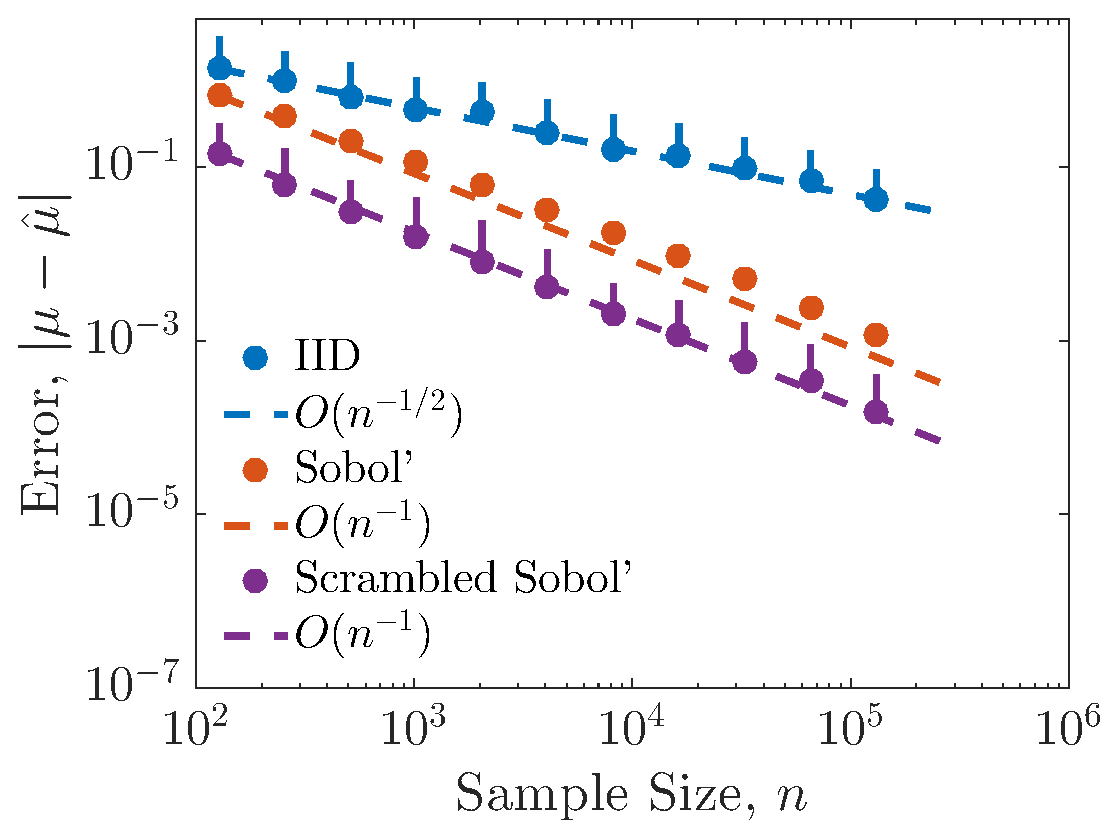
\includegraphics[width = 7cm]{ProgramsImages/AsianCallIIDUSobolSobol.eps}
	\end{tabular}
	
\end{frame}

\begin{frame}<1>[label = Summary]
	\setbeamercovered{transparent=30}
	\frametitle{Summary \uncover<1-4>{So Far}}
	\vspace{-7ex}
	\begin{equation*}
	\redroundmathbox{\mu - \hmu =\, ?} 
	\end{equation*}
	\vspace{-8ex}
	\begin{center}
		\begin{tabular}{>{\centering}p{0.45\textwidth}>{\centering}p{0.5\textwidth}}
			\alert{Reality} & \alert{Error Analysis (Theory)} \tabularnewline 
			What is &  What we think it should be
		\end{tabular}
	\end{center}
	\vspace{-3ex}		
	\begin{itemize}
		\item<1,5| only@1-> \alert{Trio identity}: $\redroundmathbox{\mu - \hmu = \algn(f, \nu - \hnu) \, \disc(\nu - \hnu) \, \Var(f)}$---keep all  terms
		\item<1,5| only@1-> Big data may not eliminate the need for \alert{proper sampling}---simple random sampling beats haphazard sampling
		\item<1,5| only@1-> \alert{Low discrepancy} sampling beats simple random sampling
		\item<1,5| only@1-> \alert{Randomization} to remove bias can improve convergence rate
		\item<2,5| only@2-> \alert{Bayesian cubature} provides even faster convergence rates with confidence intervals, but requires time consuming calculations
		\item<3,5|only@3-> Error may be \alert{dimension-independent} if the dependence of $f(x_1, x_2, \ldots)$ on $x_k$  decays quickly as $k$ increases
		\item<4-|only@4-> \alert{Changing the integrand} while leaving $\mu$ unchanged can reduce error
		\item<5 | only@5-> There are data-based \alert{stopping criteria} with theoretical justification
	\end{itemize}
\end{frame}



\begin{frame}
	\frametitle{Bayesian Trio Identity}
	\vspace*{-4ex}
	\alert{Random} $f$ postulated by \ocite{Dia88a}, \ocite{OHa91a}, \ocite{Rit00a}, \ocite{RasGha03a} and others:  $f \sim \GP (0, s^2C_{\vtheta})$,  a \alert{Gaussian process} from the sample space $\cf$ with zero mean and covariance kernel, $s^2C_{\vtheta}$, $C_{\vtheta}:\cx \times \cx \to \reals$. The \alert{scale parameter}, $s$, and \alert{shape parameter}, $\vtheta$, should be estimated.  	 Then 
	\vspace{-1ex}
	\begin{align*}
	%\mu - \hmu & \big \vert \{f(\vx_i )= y_i\}_{i=1}^n \sim \cn \bigl( \vy^T (\mC^{-1}\vc - \vw), s^2(c_0 - \vc ^T \mC^{-1} \vc) \bigr) \\
	c_0 & = \int_{\cx^2} C(\vx,\vt) \, \nu(\dif \vx) \nu(\dif \vt), \qquad \vc = \biggl( \int_{\cx} C(\vx_i,\vt) \,\nu(\dif \vt) \biggr)_{i=1}^n \\
	\mC & = \bigl( C(\vx_i,\vx_j) \bigr)_{i,j=1}^n, \qquad \vw = \bigl(w_i \bigr)_{i=1}^n,  \quad \vone^T \vw \text{ may be } \ne 1\\
	\redroundmathbox{\mu - \hmu} 
	& = \redroundmathbox{\displaystyle%
		\underbrace{\frac{ \int_{\cx} f(\vx) \, (\nu - \hnu)(\dif\vx)}{s \sqrt{c_0 - 2 \vc^T \vw + \vw^T \mC \vw}}}_{\textstyle \algn^\Ba(f,\nu - \hnu)} \, 
		\underbrace{\sqrt{c_0 - 2 \vc^T \vw + \vw^T \mC \vw}}_{\textstyle\disc^\Ba(\nu - \hnu)} \, \underbrace{s}_{\textstyle\Var^\Ba(f)}}
	\end{align*}
	\vspace{-3ex}
	\begin{itemize}
		\item 	$\vw =  \mC^{-1}\vc$ minimizes  $\disc^\Ba(\nu - \hnu)$ \\
		\hspace{1.5cm} makes $\algn^\Ba(f,\nu - \hnu) \big \vert \{f(\vx_i )= y_i\}_{i=1}^n \sim \cn (0,1)$ 
	\item $\disc^\Ba(\nu - \hnu) =  \disc^\Dt(\nu - \hnu)$  if  $C_{\vtheta} = K$		
	\end{itemize}
		
\end{frame}



\begin{frame}<1>[label=BayesCub]
	\setbeameruncoveredtransp
	\frametitle{Bayesian Cubature \hfill \uncover<2->{Deterministic Interpretation}}
	\vspace{-7.8ex}
	\[
	\begin{array}{rcl}
		f  \sim \GP (0, s^2 C_{\vtheta}) & & \uncover<2->{f \in \cf \text{ w/ reproducing kernel } K_{\vtheta}} \tabularnewline \toprule
		\multicolumn{3}{c}{\abs{\mu - \hmu} \le \text{ width}} \tabularnewline
		\text{with } 99\% \text{ confidence}&& \uncover<3->{\text{if }  \Var^{\Dt}(f - \tf_{\vy}) \le \frac{2.58}{\alert{\sqrt{n}}} \Var^{\Dt}(\tf_{\vy}) }\tabularnewline
		 2.58\sqrt{\bigl (c_{\hvtheta,0} - \vc_{\hvtheta}^T  \mC_{\hvtheta}^{-1} \vc_{\hvtheta}\bigr) \, \frac {\vy^T \mC_{\hvtheta}^{-1}  \vy}{\alert{n}} } &
		 \shortleftarrow\text{\!width}\uncover<2->{\!\shortrightarrow}&
		 \uncover<2->{\text{\alert<2>{replace} } C_{\vtheta} \text{ by } K_{\vtheta}}
		  \tabularnewline 
		  = 2.58 \disc^{\Ba}(\nu - \hnu) \Var^{\Ba}(f) &&  \uncover<3->{=\frac{2.58}{\alert{\sqrt{n}}}\disc^{\Dt}(\nu - \hnu) \Var^{\Dt}(\alert{\tf_{\vy}}) } \tabularnewline
		  \multicolumn{3}{c}{\vy = \bigl(f(\vx_i)\bigr)_{i=1}^n} \tabularnewline[0.5ex]
		  && \uncover<3->{\tf_{\vy} = \text{minimum norm interpolant}} \tabularnewline
		  \mC_{\hvtheta}^{-1} \vc_{\hvtheta} & \leftarrow \vw \uncover<2->{\rightarrow}& \uncover<2->{\text{\alert<2>{replace} } C_{\vtheta} \text{ by } K_{\vtheta}} \tabularnewline
	  \argmin_{\vtheta} \frac{\vy^T \mC_{\vtheta}^{-1} \vy}{[\det(\mC_{\vtheta}^{-1})]^{1/n}} & \leftarrow 	\hvtheta  \uncover<2->{\rightarrow} &  \uncover<2->{\text{\alert<2>{replace} } C_{\vtheta} \text{ by } K_{\vtheta}} \tabularnewline
	  \text{estimate $s$ and $\vtheta$ by MLE} & & \uncover<3->{ = \argmin_{\vtheta}  \vol \bigl(\bigl\{ \vz \in \reals^n : \tabularnewline 
	  	&& \qquad\quad \Var^{\Dt}_{\vtheta}(\tf_{\vz}) \le \Var^{\Dt}_{\vtheta}(\tf_{\vy}) \bigr\} \bigr ) }
	\end{array}
	\]
	\only<1>{\qquad \alert{Nice:\quad}$
		\begin{array}{c@{\quad}ccccc}
		\vy, \, \mC_{\vtheta} & \vw & \hmu & \text{width}& \hvtheta  \tabularnewline
		\toprule
		47 \vy, \, 29 \mC_{\vtheta} & \vw & 47 \hmu & 47 \text{width} & \hvtheta 
		\end{array}$}
	\only<3->{%
		\\[-2ex]
		\begin{tabular}{m{2.4cm}@{}m{9.2cm}}
	\quad \alert{Unfortunately: }  & 
	\begin{itemize}\setlength{\itemsep}{-0.3ex}
  			\item Requires $\Order(n^3)$ operations to compute $\mC_{\vtheta}^{-1}$
			\item Ill-conditioning for smoother kernels (faster convergence)
			\item Might not integrate constants exactly
	\end{itemize} \end{tabular}}
	
\end{frame}
	
\begin{frame} \frametitle{Multivariate Normal Probability}
	\vspace{-8ex}
	\begin{tabular}{m{8.5cm}m{3cm}}
		\begin{equation*}
		\mu = \int_{[\va,\vb]} \frac{\exp\bigl(- \frac 12 \vt^T \mSigma^{-1} \vt \bigr)}{\sqrt{(2 \pi)^d \det(\mSigma)}} \, \dif \vt \
		\overset{\text{\smallocite{Gen93}}}{=} \ \int_{[0,1]^{d-1}} f(\vx) \, \dif \vx 
		\end{equation*}
		& \GaussPict
	\end{tabular}
	\vspace{-3ex}
	
	\centerline{\redroundmathbox{\mu - \hmu = 
			\begin{Bmatrix} \uncover<2->{\cos(f,\text{error rep}) \, \disc^\Dt(\nu - \hnu) \, \Var^\Dt(f)} \\
				\uncover<2->{\algn^\Rn(f,\nu - \hnu) \,  \disc^\Rn(\nu - \hnu) \, \Var^\Dt(f)}  \\
				\algn^\Ba(f,\nu - \hnu) \,  \disc^\Ba(\nu - \hnu) \, \Var^\Ba(f) \end{Bmatrix}}}
	
	\vspace{-2ex}
	\begin{tabular}{>{\raggedleft}m{4.5cm}>{\centering}m{7cm}}
		\vspace{-2ex}
		\only<1>{Use a product Mat\'ern kernel with modest smoothness:
			\begin{multline*}C_{\theta}(\vx,\vt) \\
			= \prod_{k=1}^d (1 + \theta\abs{x_k - t_k})\me^{-\theta\abs{x_k - t_k}}
			\end{multline*}}
		\only<2>{Smaller error using Bayesian cubature with scrambled Sobol' data sites}
		\only<3>{Confidence intervals succeed $\approx 98\%$ of the time}\only<2>{\\
		\vspace{3ex}	
	
		\noindent
		$\text{\parbox{4.5cm}{\raggedleft
				\hfill For some typical choice of \newline 
				\phantom{a}\hfill  $\va$, $\vb$, $\mSigma$, and $d=3$ \newline 
				$\mu \approx 0.6763$}}  {\color{red}\Biggr \}}$}
		
		\vspace{1.5ex}
		
		&
		\includegraphics<1>[width = 7cm]{ProgramsImages/Matern.eps}
		\includegraphics<2>[width = 7cm]{ProgramsImages/MVNIIDUSobolSobolWtSobol.eps}
		\includegraphics<3>[width = 6.5cm]{ProgramsImages/MVNSobolWtSobolErrBd.eps}
	\end{tabular}
	
\end{frame}

\againframe<2->{BayesCub}


\begin{frame}
	\frametitle{Randomized Bayesian Trio Identity}
	\vspace*{-4ex}
	$f \sim \GP (0, s^2C)$ and $\hnu$ is  \alert{random} (independent of $f$):
	\vspace{-1ex}
	\begin{align*}
	\redroundmathbox{\mu - \hmu} 
	& =  \redroundmathbox{\displaystyle%
		\underbrace{\frac{ \int_{\cx} f(\vx) \, (\nu - \hnu)(\dif\vx)}{s \sqrt{\Ex_{\hnu}\bigl(c_0 - 2 \vc^T \vw + \vw^T \mC \vw\bigr)}}}_{\textstyle \algn^{\Rn\Ba}(f,\nu - \hnu) \sim \cn ( 0, 1 )} \, 
		\underbrace{\sqrt{\Ex_{\hnu}\bigl(c_0 - 2 \vc^T \vw + \vw^T \mC \vw\bigr)}}_{\textstyle\disc^{\Rn\Ba}(\nu - \hnu)} \, \underbrace{s}_{\textstyle\Var^\Ba(f)}}
	\end{align*}
	For $\vw  = \vone/n$, and unbiased estimation:
	\[
	\disc^{\Ba\Rn}(\nu - \hnu) = \sqrt{\frac {\vone^T \tmC \vone}{n^2} - c_0 }, \qquad \tmC  = \Bigl(\Ex_{\hnu} C(\vx_i,\vx_j) \Bigr)_{i,j=1}^n
	\]	
	For some $\{\vx_i\}_{i=1}^n$, such as IID samples, scrambled nets and shifted integration lattices
	\[
	\disc^{\Ba\Rn}(\nu - \hnu) = \sqrt{ \frac {\vone^T\tvC_1}{n} - c_0 }, \qquad \tmC  = (\tvC_1, \ldots, \tvC_n)
	\]	
	which requires only $\Order(n)$ operations to evaluate \smallcite{Hic99b,HicYue00}
	
\end{frame}

\againframe<2>{Summary}

\section{Tractability}

\begin{frame}
	\frametitle{The Effect of Dimension on the Discrepancy}
	\vspace{-5ex}
   What happens when dimension, $d$, is large and but sample size, $n$, is modest?
	
	\begin{tabular}{m{6cm}>{\centering}m{5.5cm}}
	 $L^2$-discrepancy and variation:
	 \begin{multline*}
	\disc^2 =\left(\frac 43\right)^d
	 - \frac{2}{n} \sum_{i=1}^n \prod_{k=1}^d \left (\frac{3 - x_{ik}^2}{2} \right) \\ + \frac{1}{n^2}\sum_{i,j=1}^n \prod_{k = 1}^d [2 - \max(x_{ik},x_{jk})]
	  \end{multline*}
	\[ 	\Var(f) = \Biggl \lVert \biggl ( \biggl \lVert\frac{\partial^{\abs{\fu}} f}{\partial \vx_\fu} \Bigr \rvert_{\vx_{\widebar{\fu}} = \vone}\biggr\rVert_{L^2}\biggr )_{\!\!\!\fu \ne \emptyset} \Biggr \rVert_2 \]
	 & 
	 For Scrambled Sobol' points \\
	 \includegraphics[width = 5.5cm]{ProgramsImages/UnwtL2Disc.eps}
	\end{tabular}
	The constant in the $\Order(n^{-1+\epsilon})$ convergence of $\disc$ is \alert{$d$ dependent}. 
\end{frame}

\begin{frame}
	\frametitle{Pricing a Financial Derivative}
	\vspace{-7ex}
	\begin{tabular}{m{8.5cm}m{3cm}}
			\centerline{\redroundmathbox{\mu - \hmu =	\algn(f,\nu - \hnu)  \disc(\nu - \hnu) \Var(f) }  }
		& \financePict
	\end{tabular}

\ocite{PasTra95} discovered that low discrepany sampling gave significant performance gains for pricing a Collaterlized Mortgage Obligation with \alert{$d = 360$}
\end{frame}
	
	\begin{frame}
		\frametitle{Pricing an Asian Option}
		\vspace{-7ex}
		\begin{tabular}{m{8.5cm}m{3cm}}
			\begin{equation*}
			\mu = \int_{\reals^d} \text{payoff}(\vt) \, \frac{\exp\bigl(- \frac 12 \vt^T \mSigma^{-1} \vt \bigr)}{\sqrt{(2 \pi)^d \det(\mSigma)}} \, \dif \vt = \int_{[0,1]^{d}} f(\vx) \, \dif \vx 
			\end{equation*}
			& \financePict
		\end{tabular}
		\vspace{-1ex}
		
		\centerline{\redroundmathbox{\mu - \hmu =	\algn(f,\nu - \hnu)  \disc(\nu - \hnu) \Var(f) }  }
		
			\vspace{-1ex}
			\begin{tabular}{m{4.5cm}m{7cm}}
				\vspace{-1ex}
				
				\noindent
				$\text{\parbox{4.5cm}{\raggedleft
						\hfill For an Asian arithmetic mean option,  \alert{$d = 13$},
						$\mu \approx \$6.1375$}} {\color{red}\biggr \}}$
				
				\bigskip
				Scrambled Sobol' achieves $\Order(n^{-1})$ convergence for modest $n$ provided that the Brownian motion is constructed by \alert{principal component analysis (PCA)}, rather than time stepping
				&
				\includegraphics[width = 7cm]{ProgramsImages/AsianCallSobolPCADiff.eps}
			\end{tabular}
	
\end{frame}
\begin{frame}
	\frametitle{Overcoming the Curse of Dimensionality with Weights}
	\vspace{-4ex}
	\begin{itemize}
		\item 	\ocite{SloWoz98} show how inserting decaying coordinate weights yields $\Order(n^{-1+\epsilon})$ convergence \alert{independent of dimension}
		\item \ocite{CafMorOwe97} explain how quasi-Monte Carlo methods work well for \alert{low effective dimension}
		\item \ocite{NovWoz10a} cover \alert{tractability} comprehensively
	\end{itemize}
	\vspace{-7ex}
	\begin{tabular}{m{6cm}>{\centering}m{5.5cm}}
		\begin{multline*}
		\disc^2 = \prod_{k=1}^d\Bigl(1 + \frac{\alert{\gamma_k^2}}{3}\Bigr) \\
			- \frac{2}{n} \sum_{i=1}^n \prod_{k=1}^d \left (1 + \frac{\alert{\gamma_k^2}(1 - x_{ik}^2)}{2} \right) \\ + \frac{1}{n^2}\sum_{i,j=1}^n \prod_{k = 1}^d [1 + \alert{\gamma_k^2}( 1 - \max(x_{ik},x_{jk}))]
		\end{multline*}
		\vspace{-4ex}
		\begin{gather*} 	\Var(f) = \Biggl \lVert \Biggl ( \!\!\frac{1}{\alert{\gamma_{\fu}} }\biggl \lVert\frac{\partial^{\abs{\fu}} f}{\partial \vx_\fu} \Bigr \rvert_{\vx_{\widebar{\fu}} = \vone}\biggr\rVert_{L^2}\!\!\Biggr )_{\!\!\!\!\fu \ne \emptyset} \Biggr \rVert_2 \\
		\alert{\gamma_{\fu}} = \prod_{k \in \fu} \alert{\gamma_k}
		\end{gather*}
		& 
		For Scrambled Sobol' points \\ $\gamma_k^2 = k^{-3}$ \\
		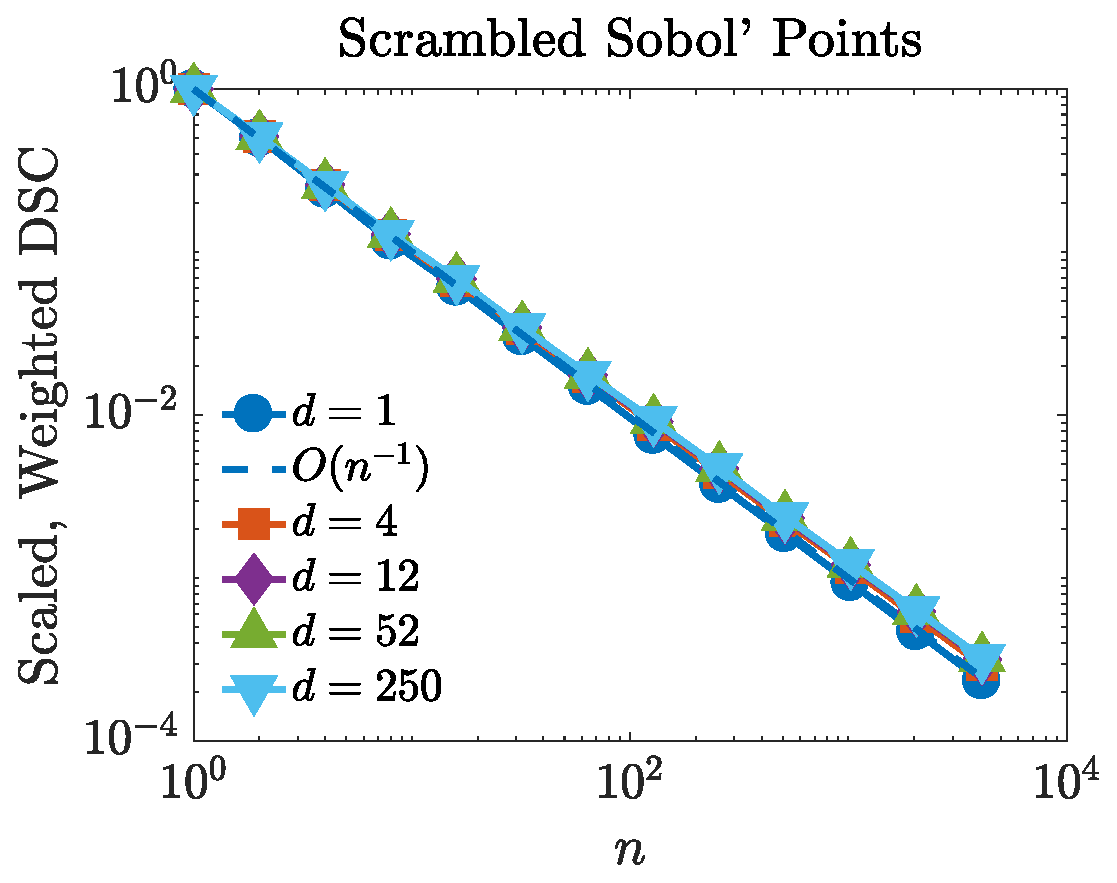
\includegraphics[width = 5.5cm]{ProgramsImages/WtL2Disc.eps}
	\end{tabular}
\end{frame}

\againframe<3>{Summary}

\section{Rewriting the Problem}

\begin{frame}
	\setbeameruncoveredtransp
	\frametitle{Reducing $\Var$}
	\vspace{-7ex}
	\begin{align*}
	\mu &= \int_{[0,1]^d} g(\vx) \, \dif \vx = \int_{[0,1]^d} f(\vx) \, \dif \vx, \qquad \nu = \text{uniform} \\
	 \redroundmathbox{\mu - \hmu(g)} & = \redroundmathbox{\algn(g,\nu - \hnu) \, \disc(\nu - \hnu) \, \Var(g)} \\
	  \redroundmathbox{\mu - \hmu(f)}& = \redroundmathbox{\algn(f,\nu - \hnu) \, \disc(\nu - \hnu) \, \Var(f)}
	\end{align*}
	Find $f$ with $\algn(f,\nu - \hnu) \Var(f) < \algn(g,\nu - \hnu) \Var(g)$.
	
	\vspace{-2ex}
	
	\begin{tabular}{m{6cm}m{5.5cm}}
		\begin{itemize}[<+->]
			\item Use \alert{PCA} instead of time differencing for Brownian motion
			\item Multivariate normal probability
			\only<2>{\vspace{-1ex}\[\begin{aligned}
			\mu & = \int_{[\va,\vb]} \frac{\exp\bigl(- \frac 12 \vt^T \mSigma^{-1} \vt \bigr)}{\sqrt{(2 \pi)^d \det(\mSigma)}} \, \dif \vt \\
			& \overset{\text{affine}}{=}  \int_{[0,1]^d} g(\vx) \, \dif \vx  \\
		& \overset{\text{\scriptsize{\ocite{Gen93}}}}{=} \int_{[0,1]^d} f(\vx) \, \dif \vx
			\end{aligned}\]}
		\item \alert{Control variates:} $f(\vx)  = g(\vx) + \vbeta^T(\vmu_{\vh} - \vh(\vx) )$ \only<3>{\\$\vbeta$ for low discrepancy sampling may be different than for IID sampling \smallcites{HicEtal03,Li16a}}
		\item Change of variables---\alert{importance sampling} and \alert{antithetic variates}
		\end{itemize}
		&
		\only<1>{\vspace{2ex}\includegraphics[width = 5.5cm]{ProgramsImages/AsianCallSobolPCADiff.eps}}
		\only<2>{\vspace{-12ex}\includegraphics<2>[width = 5.5cm]{ProgramsImages/MVNSobolGenzAff.eps}}
		\only<3>{\vspace{-4ex}\centerline{Asian Arithmetic Mean Call} 
			 \centerline{$\varepsilon = 0.0001$}
			\medskip
			\begin{tabular}{p{3cm}c}
				& Time \tabularnewline
				w/o control variates & $1.01$ s\tabularnewline
				w/ Geometric Mean Call control variate & $0.26$ s
			\end{tabular}}
	\end{tabular}
\end{frame}

\begin{frame}
	\setbeameruncoveredtransp
	\frametitle{Controlling Costs for $d \to \infty$}
	\vspace{-4ex}
	E.g., for options based on continuously monitored assets:
	\[
	\mu = \lim_{d \to \infty} \mu_d, \quad  \mu_d:= \int_{\cx_d} f_d(\vx) \, \nu_d(\dif \vx)
	\]
\vspace{-4ex}
	\begin{itemize}
		\item For $\mu \approx \hmu_{d_{\hugetext}}$, how big should $d_{\hugetext}$ be?
		\item Computational cost of evaluating $\hmu_{d}$ is typically \alert{$\Order(dn)$}
	\end{itemize}
	\vspace{-2ex}
	
	\uncover<2->{Break $f$ into pieces:
	\[
	f = f_{\emptyset} + f_{\{1\}} + f_{\{2\}} + \cdots + f_{\{1,2\}} + \cdots, \quad f_{\fu} \text{ depends only on } \vx_{\fu}, \quad f_d = \sum_{\fu \subseteq 1:d} f_{\fu}
	\]
	\vspace{-4ex}
	
	If $f_{\fu}$ gets small as $\max \{k : k \in \fu\}$ gets large, then can use \alert{fewer} samples on the pieces of the  function that are \alert{more expensive to evaluate.}
	\begin{description}[fred]
		\item[Multi-Level Monte Carlo Method:] $\hmu = \hmu(f_{d_1}) + \hmu(f_{d_2} - f_{d_1}) + \cdots + \hmu(f_{d_L} - f_{d_{L-1}}) $ \\ $d_1 < \cdots < d_L$, \smallcites{Hei01a, Gil08b, Gil14a, Gil15a, HicMGRitNiu09a, NiuHic09b};
		\smallocite{RheGly12a} remove bias\\[2ex]
		
		\item[Multivariate Decomposition Method:] $\hmu = \hmu(f_{\fu_1}) + \hmu(f_{\fu_2}) + \cdots +\hmu(f_{\fu_L})$ \\
		where the $\fu_k$ are the important coordinate indices \smallcite{Was13b}
	\end{description}}
\end{frame}


\againframe<4>{Summary}


\section{When to Stop}
\begin{frame}
	\frametitle{How Many Samples Are Needed?}
	Given  an \alert{error tolerance}, $\varepsilon$, how do we decide how many samples, $n$, are needed to make
	\[
	\redroundmathbox{\abs{\mu - \hmu} = \abs{\algn(f, \nu - \hnu)} \, \disc(\nu - \hnu) \, \Var(f)} \le \varepsilon
	\]
	\vspace{-6ex}
	\begin{itemize}
		\item \alert{Bayesian cubature} provides data-based confidence intervals for $\hmu$
		
		\item For \alert{IID Monte Carlo}, $\abs{\mu - \hmu }= \abs{\algn^{\Rn}(f, \nu - \hnu)} \std(f)/\sqrt{n}$ can be bounded with high probability assuming a bound on $\kurt(f)$ \smallcites{HicEtal14a,BayEtal14a,Jia16a}
		
		\item For \alert{digital net} (e.g., Sobol') and \alert{integration lattice} sampling, rigorous stopping criteria may be constructed in terms of the discrete Fourier Walsh/complex exponential coefficients of $f$ \smallcites{HicJim16a, JimHic16a, Li16a}
	\end{itemize}
\end{frame}

\againframe<5>{Summary}

\thankyouframe

\begin{frame}[allowframebreaks]\frametitle{References}
	\bibliography{FJH23,FJHown23}
\end{frame}

\end{document}

